\chapter{Metode Kembangan}

Terdapat 2 metode yang penulis kembangkan. Metode pertama adalah model LSTM Autoencoder yang merupakan metode umum digunakan data engineer untuk anomaly detection. Metode kedua adalah model Bayesian Probability yang merupakan model inovasi buatan penulis sendiri.

\section{LSTM Autoencoder}

Long-short term memory (LSTM) neural network adalah arsitektur jenis khusus dari recurrent neural network (RNN) yang dapat mengingat informasi dalam jangka waktu yang panjang.

LSTM cocok untuk mengklasifikasi, memproses, dan memprediksi data time series, karena mungkin terdapat jeda waktu yang tidak diketahui di antara peristiwa penting pada time series.

\begin{figure}[h]
    \centering
    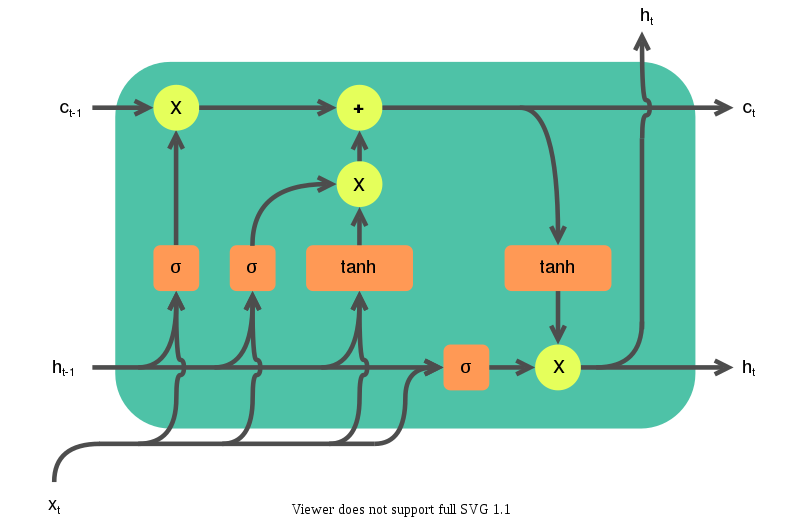
\includegraphics[width=0.6\textwidth]{resources/LSTM/LSTM_cell.png}
    \caption{Satu sel LSTM}
\end{figure}

LSTM Autoencoder adalah model neural network yang menggunakan LSTM sebagai hidden layernya untuk belajar menyalin input ke output. Autoencoder terdiri dari dua bagian, yaitu encoder yang menyalin input menjadi kode dan decoder yang menyalin kode menjadi output.

\begin{figure}[h]
    \centering
    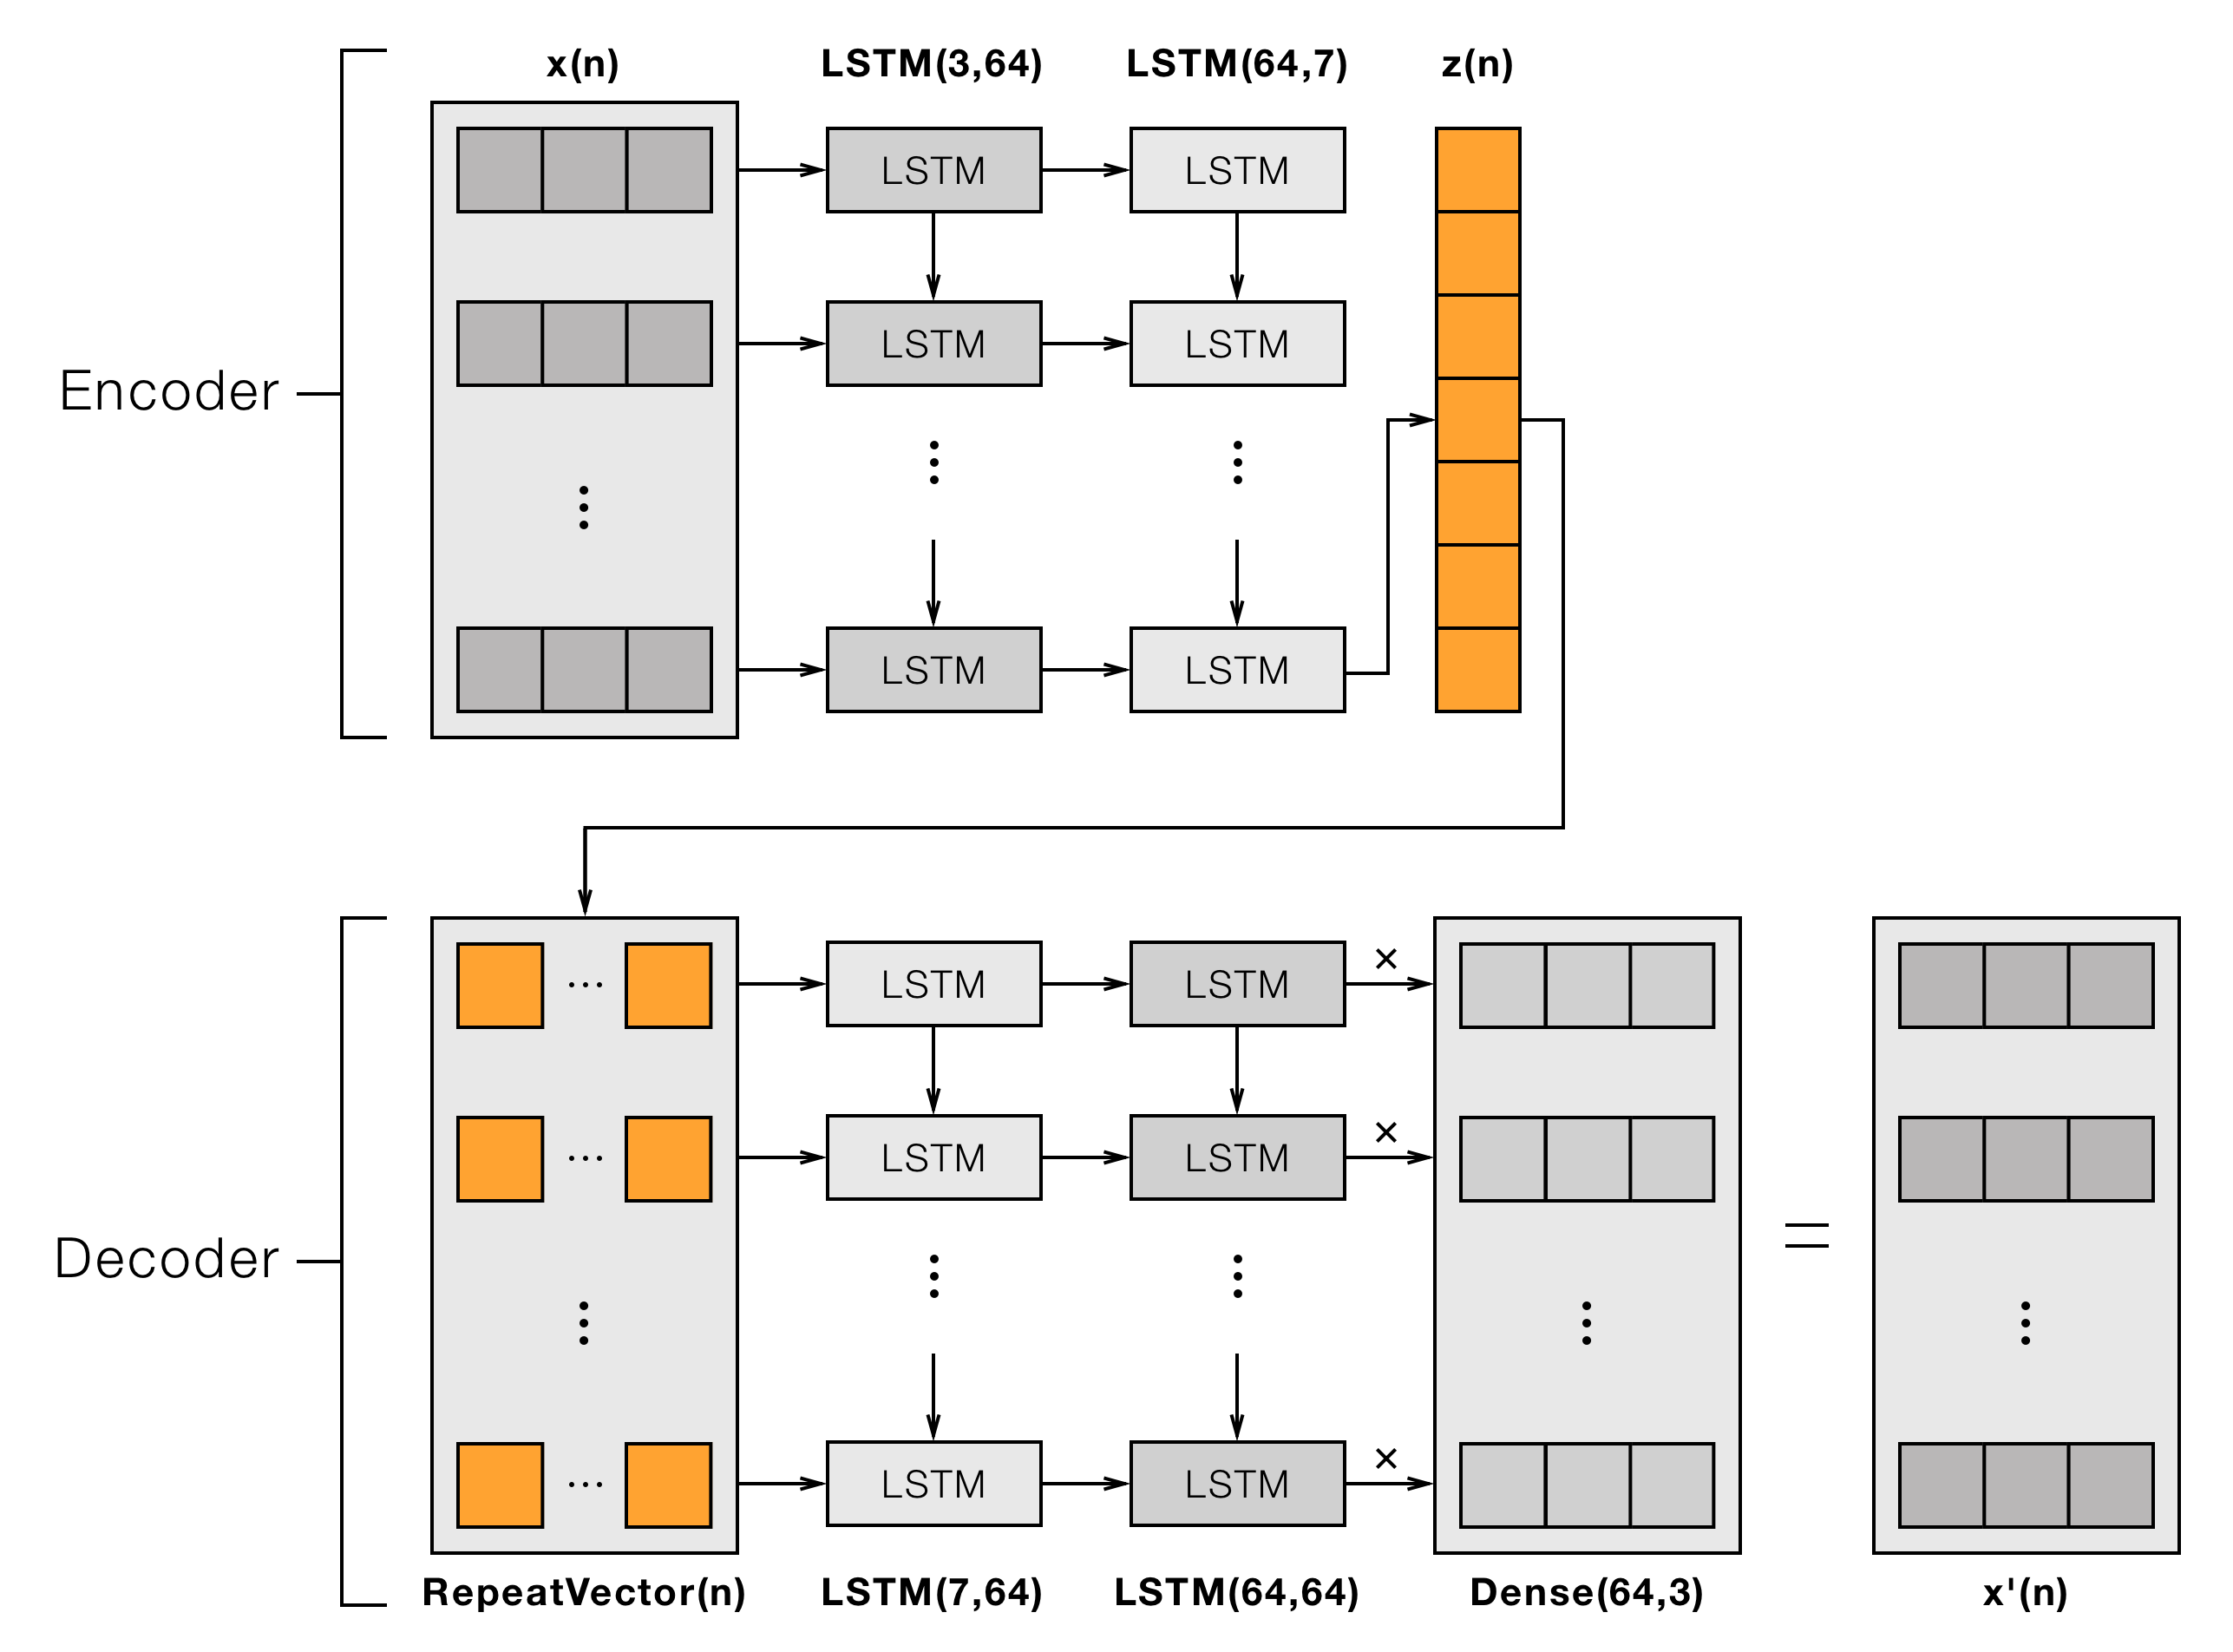
\includegraphics[width=0.8\textwidth]{resources/LSTM/lstm_ae.png}
    \caption{LSTM Autoencoder}
\end{figure}

Dengan begitu autoencoder dapat mempelajari fitur-fitur yang dimiliki input sehingga dapat melakukan prediksi, dan jika menggunakan LSTM sebagai hidden layernya maka dapat digunakan untuk memprediksi input berupa time series.

Karena lebih cocok untuk data time series, maka diharapkan model ini mampu memberikan hasil lebih baik dari model acuan.

Model LSTM Autoencoder didefinisikan melalui class \texttt{Encoder} dan \texttt{Decoder} yang kemudian digabung pada class \texttt{RecurrentAutoencoder}.

\section{Bayesian Probability}
\subsection{Idea and Concept}

Ide awal untuk menggunakan model Bayesian untuk anomaly detection berasal dari konsep anomaly detection menggunakan pendekatan identifikasi data outlier. Beberapa metode umum untuk mendeteksi data outlier seperti K-Means Clustering dan Isolation Forest menggunakan konsep pengelompokkan data atau clustering data. Sehingga akan diperoleh data-data yang berada didalam cluster tersebut dan data yang berada diluar cluster diidentifikasi sebagai outlier.

Terlihat disini bahwa pendekatan clustering ini mirip dengan model Bayesian untuk respon biner. Asumsikan setiap data memiliki suatu probabilitas apakah data tersebut termasuk pada cluster normal ataukah outlier. Dengan begitu, dapat diekspektasi distribusi probabilitas akan memiliki kontur lingkaran. Semakin dekat suatu data dengan pusat lingkaran, maka data tersebut semakin likely merupakan data normal. Pusat lingkaran akan menjadi titik dengan probabilitas suatu data merupakan data normal sebesar 1, artinya pusat lingkaran adalah titik data ideal dari kondisi normal dataset, dalam kasus ini yaitu hasil pengukuran ideal dari sensor-sensor pada sistem mesin. Sebaliknya, semakin jauh dari pusat lingkaran maka akan semakin unlikely data tersebut adalah data normal, atau dalam arti lain: data tersebut semakin likely merupakan anomaly.

\subsection{Deriving the Maths}

Definisikan data yang menjadi input model ini adalah 2 komponen utama dari hasil Principal Componen Analysis (PCA). Hal ini karena semakin tinggi dimensi data input, model akan semakin kompleks. Oleh karena itu data yang akan digunakan adalah komponen pertama PCA (pc1) sebagai $x_0$ dan komponen kedua PCA (pc2) sebagai $x_1$.

\begin{equation}
    \mathbf{x_n}=\begin{bmatrix} x_0 \\ x_1 \end{bmatrix}
\end{equation}

Sesuai ekspektasi awal, distribusi probabilitas akan memiliki kontur lingkaran. Maka, diperlukan 2 buah fungsi. Pertama adalah fungsi yang memetakan $\mathbf{x_n}$ ke suatu nilai dengan kontur lingkaran. Kedua adalah fungsi yang memetakan nilai kontur tersebut ke dalam range $[0,1]$, karena probabilitas hanya bernilai diantara 0 hingga 1.

Definisikan fungsi pertama sebagai
\begin{equation}
    f(\mathbf{w,x_n})=(w_0+x_0)^2+(w_1+x_1)^2 \label{fungsi_f}
\end{equation}
dengan
\begin{equation}
    \mathbf{w}=\begin{bmatrix} w_0 \\ w_1 \end{bmatrix}
\end{equation}
sebagai vektor parameter yang menentukan bentuk dan posisi kontur. Kemudian, dengan menetapkan data normal memiliki respon $t_n=1$ dan data anomaly memiliki respon $t_n=0$, didefinisikan fungsi kedua sebagai
\begin{equation*}
    P(T_n=1|\mathbf{x_n}, \mathbf{w}) = \frac{1}{1+f(\mathbf{w,x_n})}
\end{equation*}
Untuk penyederhanaan penulisan, $f(\mathbf{w,x_n})$ akan disingkat sebagai $f$ dan $P(T_n=1|\mathbf{x_n}, \mathbf{w})$ sebagai $P_n$.
\begin{equation}
    P_n = \frac{1}{1+f}
\end{equation}
Konsep model bayesian menggunakan pendekatan dengan memisalkan suatu sampling dengan rasio sukses $p = P(T_n=1|\mathbf{x_n},\mathbf{w})$, sampling dilakukan hanya 1 kali ($N=1$) untuk total sukses sebanyak $Y_N=t_n$. Maka dengan distribusi binomial
\begin{equation*}
    P(T_n=t_n|\mathbf{x_n},\mathbf{w})=\mathbf{Binomial}(Y_N=y|p,N)=\frac{N!}{(N-y)!y!}p^{y}(1-p)^{N-y}
\end{equation*}
\begin{equation*}
    P(T_n=t_n|\mathbf{x_n},\mathbf{w})=P(T_n=1|x_n,w)^{t_n}\left(1-P(T_n=1|x_n,w)\right)^{1-t_n}
\end{equation*}
\begin{equation}
    P(T_n=t_n|\mathbf{x_n},\mathbf{w})=P_n^{t_n}\left(1-P_n)\right)^{1-t_n} \label{likelihood}
\end{equation}
Berdasarkan data yang diketahui ($\mathbf{x_n}$ dan $t_n$), dengan asumsi seluruh data saling independen, dapat dihitung probability likelihood sebagai
\begin{equation*}
    p(t|\mathbf{X},\mathbf{w})=\prod_{n=1}^{N} P(T_n=t_n|\mathbf{x_n},\mathbf{w})
\end{equation*}
\begin{equation}
    p(t|\mathbf{X},\mathbf{w})=\prod_{n=1}^{N} P_n^{t_n}\left(1-P_n)\right)^{1-t_n}
\end{equation}
Persamaan probabilitas bayes adalah
\begin{equation}
    p(\mathbf{w}|\mathbf{X},t)=\frac{p(t|\mathbf{X},\mathbf{w})p(\mathbf{w})}{p(t|\mathbf{X})}
\end{equation}
Pada kasus anomaly detection, model dilatih untuk mencari parameter $\mathbf{w}$ yang terbaik dalam memetakan seluruh data yang diasumsikan data normal sebagai data yang likely merupakan data normal. Model bayesian memodelkan seluruh variabel sebagai variabel bebas yang terdistribusi dengan suatu probabilitas. Maka, parameter $\mathbf{w}$ yang terbaik adalah ekspektasi dari distribusi probabilitas $p(\mathbf{w}|\mathbf{X},t)$. Sehingga, parameter $\mathbf{w}$ terbaik akan berada pada titik maksimum dari $p(\mathbf{w}|\mathbf{X},t)$. Oleh karena itu, $\mathbf{w}$ terbaik dapat ditentukan dengan menyelesaikan
\begin{equation*}
    \frac{\partial{p(\mathbf{w}|\mathbf{X},t)}}{\partial{\mathbf{w}}} = 0
\end{equation*}
\begin{equation*}
    \frac{\partial}{\partial{\mathbf{w}}} \frac{p(t|\mathbf{X},\mathbf{w})p(\mathbf{w})}{p(t|\mathbf{X})} = 0
\end{equation*}
Karena $p(t|\mathbf{X})$ independen terhadap $\mathbf{w}$, Maka
\begin{equation}
    \frac{\partial}{\partial{\mathbf{w}}} p(t|\mathbf{X},\mathbf{w})p(\mathbf{w}) = 0 \label{ODE}
\end{equation}
Asumsikan parameter $\mathbf{w}$ terdistribusi normal
\begin{equation}
    p(\mathbf{w})=\mathcal{N}_\mathbf{w}\left(0,\sigma^2\mathbf{I}\right)=\mathcal{N}_{w_1}\left(0,\sigma^2\right)\mathcal{N}_{w_2}\left(0,\sigma^2\right) \label{prior}
\end{equation}
Maka, dari persamaan \ref{likelihood} dan \ref{prior}, persamaan \ref{ODE} menjadi
\begin{equation}
    \frac{\partial{}}{\partial{\mathbf{w}}} \left(p(\mathbf{w})\prod_{n=1}^{N} P_n^{t_n}\left(1-P_n\right)^{1-t_n}\right)=0
\end{equation}
Persamaan ini sulit diselesaikan. Namun dengan mengambil logaritma natural kedua sisi akan diperoleh
\begin{equation*}
    \frac{\partial{}}{\partial{\mathbf{w}}} \left(\ln{\left[p(\mathbf{w})\prod_{n=1}^{N} P_n^{t_n}\left(1-P_n\right)^{1-t_n}\right]}\right)=0
\end{equation*}
\begin{equation}
    \frac{\partial{}}{\partial{\mathbf{w}}}\left(\ln{\left[ p(\mathbf{w}) \right]}\right) + \frac{\partial{}}{\partial{w}} \left(\ln{\left[ \prod_{n=1}^{N} P_n^{t_n}\left(1-P_n\right)^{1-t_n}\right] }\right)=0
\end{equation}
Untuk suku pertama:
\begin{equation*}
\ln{\left[ p(\mathbf{w}) \right]} = \ln{\left[ \mathcal{N}_{w_1}\left(0,\sigma^2\right)\mathcal{N}_{w_2}\left(0,\sigma^2\right) \right]}
\end{equation*}
\begin{equation*}
\ln{\left[ p(\mathbf{w}) \right]}=\ln{\left[ \frac{1}{\sqrt{2\pi\sigma^2}}e^{-\frac{w_1^2}{2\sigma^2}} \frac{1}{\sqrt{2\pi\sigma^2}}e^{-\frac{w_2^2}{2\sigma^2}} \right]}
\end{equation*}
\begin{equation*}
\ln{\left[ p(\mathbf{w}) \right]}=-\frac{w_1^2+w_2^2}{2\sigma^2}-\ln\left({2\pi\sigma^2}\right)
\end{equation*}
\begin{equation}
\frac{\partial{}}{\partial{\mathbf{w}}}\left(\ln{\left[ p(\mathbf{w}) \right]}\right)=-\frac{\mathbf{w^T}}{\sigma^2} \label{ODE_1st_term}
\end{equation}

dan untuk suku kedua:
\begin{equation*}
    \ln{\left[ \prod_{n=1}^{N} P_n^{t_n}\left(1-P_n\right)^{1-t_n} \right] }=\sum_{n=1}^{N} \ln{ \left[ P_n^{t_n}\left(1-P_n\right)^{1-t_n} \right] }
\end{equation*}
\begin{equation*}
    \ln{\left[ \prod_{n=1}^{N} P_n^{t_n}\left(1-P_n\right)^{1-t_n} \right] }=\sum_{n=1}^{N} t_n\ln{(P_n)} + (1-t_n)\ln{(1-P_n)}
\end{equation*}
Variabel $t_n$ adalah data yang diketahui dari dataset, ini berarti $t_n$ independen dari $\mathbf{w}$. Sehingga:
\begin{equation}
    \frac{\partial}{\partial{\mathbf{w}}} \ln{\left[ \prod_{n=1}^{N} P_n^{t_n}\left(1-P_n\right)^{1-t_n} \right] } = \sum_{n=1}^{N} t_n \frac{\partial}{\partial{\mathbf{w}}}\ln{(P_n)} + (1-t_n) \frac{\partial}{\partial{\mathbf{w}}} \ln{(1-P_n)} \label{ODE_2nd_term}
\end{equation}
Selesaikan dahulu suku $\frac{\partial{P_n}}{\partial{\mathbf{w}}}$
\begin{equation*}
    \frac{\partial{P_n}}{\partial{\mathbf{w}}} = \frac{\partial{P_n}}{\partial{f}} \frac{\partial{f}}{\partial{\mathbf{w}}} = \frac{\partial}{\partial{f}} \left( \frac{1}{1+f} \right) \frac{\partial{f}}{\partial{\mathbf{w}}}
\end{equation*}
Definisikan suatu fungsi $g(f)$ sebagai
\begin{equation}
    g(f) = \frac{\partial}{\partial{f}} \left( \frac{1}{1+f} \right) = -\frac{1}{(1+f)^2} \label{fungsi_g}
\end{equation}
Untuk mempersingkat penulisan, fungsi $g(f)$ akan disingkat menjadi $g$. Diperoleh
\begin{equation}
    \frac{\partial{P_n}}{\partial{\mathbf{w}}} = g \frac{\partial{f}}{\partial{\mathbf{w}}} \label{dPndw_vec}
\end{equation}
dengan
\begin{equation}
    \frac{\partial{f}}{\partial{\mathbf{w}}} = \begin{bmatrix} \frac{\partial{f}}{\partial{w_0}} && \frac{\partial{f}}{\partial{w_1}}\end{bmatrix} \label{dfdw_vec}
\end{equation}
dan dari persamaan \ref{fungsi_f}, dapat diperoleh
\begin{equation}
    \frac{\partial{f}}{\partial{w_n}} = 2(w_n+x_n) \label{dfdwn}
\end{equation}
Maka, dengan persamaan \ref{dPndw_vec} persamaan \ref{ODE_2nd_term} menjadi
\begin{align*}
    \frac{\partial}{\partial{\mathbf{w}}} \ln{\left[ \prod_{n=1}^{N} P_n^{t_n}\left(1-P_n\right)^{1-t_n} \right] } & = \sum_{n=1}^{N} t_n \frac{\partial}{\partial{\mathbf{w}}}\ln{(P_n)} + (1-t_n) \frac{\partial}{\partial{\mathbf{w}}} \ln{(1-P_n)} \\
    & = \sum_{n=1}^{N} t_n \frac{1}{P_n} \frac{\partial{P_n}}{\partial{\mathbf{w}}} - (1-t_n) \frac{1}{(1-P_n)} \frac{\partial{P_n}}{\partial{\mathbf{w}}} \\
    & = \sum_{n=1}^{N} t_n \frac{1}{P_n} g \frac{\partial{f}}{\partial{\mathbf{w}}} - (1-t_n) \frac{1}{(1-P_n)} g \frac{\partial{f}}{\partial{\mathbf{w}}} \\
    & = \sum_{n=1}^{N} \frac{(t_n-P_n)g}{P_n(1-P_n)} \frac{\partial{f}}{\partial{\mathbf{w}}}
\end{align*}
dan dengan \ref{ODE_1st_term} didapatkan persamaan \ref{ODE} menjadi
\begin{equation}
    -\frac{\mathbf{w^T}}{\sigma^2}+\sum_{n=1}^{N} \frac{(t_n-P_n)g}{P_n(1-P_n)} \frac{\partial{f}}{\partial{\mathbf{w}}}=0 \label{ODE_final}
\end{equation}
Persamaan ini tidak dapat diselesaikan secara analitik. Namun dengan metode numerik Newton-Rhapson, solusi $\mathbf{w}$ dapat diperoleh dengan mendefinisikan
\begin{equation}
    \mathbf{F^T}(\mathbf{w}) = -\frac{\mathbf{w^T}}{\sigma^2}+\sum_{n=1}^{N} \frac{(t_n-P_n)g}{P_n(1-P_n)} \frac{\partial{f}}{\partial{\mathbf{w}}} \label{F_vec}
\end{equation}
Maka persamaan \ref{ODE_final} terpenuhi pada kondisi $\mathbf{F^T}(\mathbf{w}) = 0$ yang dapat ditentukan dengan menebak suatu $\mathbf{w}$ awal dan melakukan iterasi
\begin{equation}
    \mathbf{w}_{i+1} = \mathbf{w}_{i} - \mathbf{H}^{-1}\mathbf{F}(\mathbf{w}) \label{iter}
\end{equation}
Dengan $\mathbf{H}$ adalah Hessian matrix
\begin{equation}
    \mathbf{H} = 
    \begin{bmatrix}
    \frac{\partial{F_0}}{\partial{w_0}} & \frac{\partial{F_0}}{\partial{w_1}} \\
    \frac{\partial{F_1}}{\partial{w_0}} & \frac{\partial{F_1}}{\partial{w_1}} 
    \end{bmatrix} \label{H_mat}
\end{equation}
dan $F_0$ serta $F_1$ adalah komponen-komponen dari vektor $\mathbf{F}(\mathbf{w})$. Elemen-elemen pada matrix hessian dapat ditentukan dengan
\begin{equation}
    \frac{\partial{F_m}}{\partial{w_n}} = - \frac{\delta_{mn}}{\sigma^2} + \sum_{n=1}^{N} \left(
    \frac{1}{P_n(1-P_n)}
    \left[
    (t_n-P_n) \frac{\partial{g}}{\partial{w_n}} - g \frac{\partial{P_n}}{\partial{w_n}}
    \right]
    - \frac{(t_n-P_n)g}{P_n^2(1-P_n)^2} (1-2P_n) \frac{\partial{P_n}}{\partial{w_n}}
    \right)
    \frac{\partial{f}}{\partial{w_m}} + \frac{(t_n-P_n)g}{P_n(1-P_n)} \frac{\partial^2{f}}{\partial{w_n}\partial{w_m}} \label{dFn_dwm}
\end{equation}
dengan $\delta_{mn}$ adalah fungsi delta kronecker. Kemudian persamaan \ref{fungsi_g} dan \ref{fungsi_f} dapat diperoleh
\begin{equation}
    \frac{\partial{g}}{\partial{w_n}} = \frac{1}{(1+f)^3} \frac{\partial{f}}{\partial{w_n}} \label{dotg}
\end{equation}
\begin{equation}
    \frac{\partial^2{f}}{\partial{w_n}\partial{w_m}} = 2\delta_{mn} \label{ddotf}
\end{equation}


\subsection{Algorithms}

\begin{python}
    time = datetime.datetime.now()
    print("Start training at : {}".format(time))
    
    w = np.zeros(2)
    var_w = 10
    w_iter = []
    w_iter.append(w)
    maxIter = 10
    nIter = 1
    tol = 10**-6
    delta = 10**6
    while (nIter<maxIter) and (delta>tol):
        Hess = H_mat(t,w,X_scaled)
        F_vector = F_vec(t,w,X_scaled)
        dw = np.matmul(np.linalg.inv(Hess),F_vector)
        delta = sum(dw**2)
        w = w - dw
        print("nIter = %d, delta=%.2e"%(nIter,delta))
        w_iter.append(w)
        nIter += 1
    
    time = datetime.datetime.now()
    print("Done training at : {}".format(time))

\end{python}
